\documentclass[11pt,twoside,letterpaper]{article}
\newcommand{\reporttitle}{Lab 1: Sensor data processing for mobile robots}
\newcommand{\reportauthorOne}{Adams, Hunter}
\newcommand{\cidOne}{20997503}
\newcommand{\reportauthorTwo}{Chen, Joe}
\newcommand{\cidTwo}{20998545}
\newcommand{\reportauthorThree}{Wielowieyski, Jacob}
\newcommand{\cidThree}{21004619}
\newcommand{\robotNumber}{7}
\newcommand{\stationNumber}{\rule{2cm}{0.4pt}}
\date{October 19, 2026}
%%%%%%%%%%%%%%%%%%%%%%%%%%%%%%%%%%%%%%%%%
% University Assignment Title Page 
% LaTeX Template
% Version 1.0 (27/12/12)
%
% This template has been downloaded from:
% http://www.LaTeXTemplates.com
%
% Original author:
% WikiBooks (http://en.wikibooks.org/wiki/LaTeX/Title_Creation)
%
% License:
% CC BY-NC-SA 3.0 (http://creativecommons.org/licenses/by-nc-sa/3.0/)
% 
% Instructions for using this template:
% This title page is capable of being compiled as is. This is not useful for 
% including it in another document. To do this, you have two options: 
%
% 1) Copy/paste everything between \begin{document} and \end{document} 
% starting at \begin{titlepage} and paste this into another LaTeX file where you 
% want your title page.
% OR
% 2) Remove everything outside the \begin{titlepage} and \end{titlepage} and 
% move this file to the same directory as the LaTeX file you wish to add it to. 
% Then add \input{./title_page_1.tex} to your LaTeX file where you want your
% title page.
%
%----------------------------------------------------------------------------------------
%	PACKAGES AND OTHER DOCUMENT CONFIGURATIONS
%----------------------------------------------------------------------------------------
\usepackage{ifxetex}
\usepackage{textpos}
\usepackage{natbib}
\usepackage{kpfonts}
\usepackage[letterpaper,hmargin=2.8cm,vmargin=2.0cm,includeheadfoot]{geometry}
\usepackage{ifxetex}
\usepackage{stackengine}
\usepackage{tabularx,longtable,multirow,subfigure,caption}%hangcaption
\usepackage{fncylab} %formatting of labels
\usepackage{fancyhdr}
\usepackage{color}
\usepackage[tight,ugly]{units}
\usepackage{url}
\usepackage{float}
\usepackage[english]{babel}
\usepackage{amsmath}
\usepackage{graphicx}
\usepackage[colorinlistoftodos]{todonotes}
\usepackage{dsfont}
\usepackage{epstopdf} % automatically replace .eps with .pdf in graphics
\usepackage{natbib}
\usepackage{backref}
\usepackage{array}
\usepackage{latexsym}
\usepackage{etoolbox}

\usepackage{enumerate} % for numbering with [a)] format 



\ifxetex
\usepackage{fontspec}
\setmainfont[Scale=.8]{OpenDyslexic-Regular}
\else
\usepackage[pdftex,pagebackref,hypertexnames=false,colorlinks]{hyperref} % provide links in pdf
\hypersetup{pdftitle={},
  pdfsubject={}, 
  pdfauthor={\reportauthorOne},
  pdfkeywords={}, 
  pdfstartview=FitH,
  pdfpagemode={UseOutlines},% None, FullScreen, UseOutlines
  bookmarksnumbered=true, bookmarksopen=true, colorlinks,
    citecolor=black,%
    filecolor=black,%
    linkcolor=black,%
    urlcolor=black}
\usepackage[all]{hypcap}
\fi

\usepackage{tcolorbox}

% various theorems
\usepackage{ntheorem}
\theoremstyle{break}
\newtheorem{lemma}{Lemma}
\newtheorem{theorem}{Theorem}
\newtheorem{remark}{Remark}
\newtheorem{definition}{Definition}
\newtheorem{proof}{Proof}

% example-environment
\newenvironment{example}[1][]
{ 
\vspace{4mm}
\noindent\makebox[\linewidth]{\rule{\hsize}{1.5pt}}
\textbf{Example #1}\\
}
{ 
\noindent\newline\makebox[\linewidth]{\rule{\hsize}{1.0pt}}
}



%\renewcommand{\rmdefault}{pplx} % Palatino
% \renewcommand{\rmdefault}{put} % Utopia

\ifxetex
\else
\renewcommand*{\rmdefault}{bch} % Charter
\renewcommand*{\ttdefault}{cmtt} % Computer Modern Typewriter
%\renewcommand*{\rmdefault}{phv} % Helvetica
%\renewcommand*{\rmdefault}{iwona} % Avant Garde
\fi

\setlength{\parindent}{0em}  % indentation of paragraph

\setlength{\headheight}{14.5pt}
\pagestyle{fancy}
\fancyfoot[ER,OL]{\thepage}%Page no. in the left on
                                %odd pages and on right on even pages
\fancyfoot[OC,EC]{\sffamily }
\renewcommand{\headrulewidth}{0.1pt}
\renewcommand{\footrulewidth}{0.1pt}
\captionsetup{margin=10pt,font=small,labelfont=bf}


%--- chapter heading

\def\@makechapterhead#1{%
  \vspace*{10\p@}%
  {\parindent \z@ \raggedright %\sffamily
        %{\Large \MakeUppercase{\@chapapp} \space \thechapter}
        %\\
        %\hrulefill
        %\par\nobreak
        %\vskip 10\p@
    \interlinepenalty\@M
    \Huge \bfseries 
    \thechapter \space\space #1\par\nobreak
    \vskip 30\p@
  }}

%---chapter heading for \chapter*  
\def\@makeschapterhead#1{%
  \vspace*{10\p@}%
  {\parindent \z@ \raggedright
    \sffamily
    \interlinepenalty\@M
    \Huge \bfseries  
    #1\par\nobreak
    \vskip 30\p@
  }}
  



% %%%%%%%%%%%%% boxit
\def\Beginboxit
   {\par
    \vbox\bgroup
	   \hrule
	   \hbox\bgroup
		  \vrule \kern1.2pt %
		  \vbox\bgroup\kern1.2pt
   }

\def\Endboxit{%
			      \kern1.2pt
		       \egroup
		  \kern1.2pt\vrule
		\egroup
	   \hrule
	 \egroup
   }	

\newenvironment{boxit}{\Beginboxit}{\Endboxit}
\newenvironment{boxit*}{\Beginboxit\hbox to\hsize{}}{\Endboxit}



\allowdisplaybreaks

\makeatletter
\newcounter{elimination@steps}
\newcolumntype{R}[1]{>{\raggedleft\arraybackslash$}p{#1}<{$}}
\def\elimination@num@rights{}
\def\elimination@num@variables{}
\def\elimination@col@width{}
\newenvironment{elimination}[4][0]
{
    \setcounter{elimination@steps}{0}
    \def\elimination@num@rights{#1}
    \def\elimination@num@variables{#2}
    \def\elimination@col@width{#3}
    \renewcommand{\arraystretch}{#4}
    \start@align\@ne\st@rredtrue\m@ne
}
{
    \endalign
    \ignorespacesafterend
}
\newcommand{\eliminationstep}[2]
{
    \ifnum\value{elimination@steps}>0\leadsto\quad\fi
    \left[
        \ifnum\elimination@num@rights>0
            \begin{array}
            {@{}*{\elimination@num@variables}{R{\elimination@col@width}}
            |@{}*{\elimination@num@rights}{R{\elimination@col@width}}}
        \else
            \begin{array}
            {@{}*{\elimination@num@variables}{R{\elimination@col@width}}}
        \fi
            #1
        \end{array}
    \right]
    & 
    \begin{array}{l}
        #2
    \end{array}
    &%                                    moved second & here
    \addtocounter{elimination@steps}{1}
}
\makeatother

%% Fast macro for column vectors
\makeatletter  
\def\colvec#1{\expandafter\colvec@i#1,,,,,,,,,\@nil}
\def\colvec@i#1,#2,#3,#4,#5,#6,#7,#8,#9\@nil{% 
  \ifx$#2$ \begin{bmatrix}#1\end{bmatrix} \else
    \ifx$#3$ \begin{bmatrix}#1\\#2\end{bmatrix} \else
      \ifx$#4$ \begin{bmatrix}#1\\#2\\#3\end{bmatrix}\else
        \ifx$#5$ \begin{bmatrix}#1\\#2\\#3\\#4\end{bmatrix}\else
          \ifx$#6$ \begin{bmatrix}#1\\#2\\#3\\#4\\#5\end{bmatrix}\else
            \ifx$#7$ \begin{bmatrix}#1\\#2\\#3\\#4\\#5\\#6\end{bmatrix}\else
              \ifx$#8$ \begin{bmatrix}#1\\#2\\#3\\#4\\#5\\#6\\#7\end{bmatrix}\else
                 \PackageError{Column Vector}{The vector you tried to write is too big, use bmatrix instead}{Try using the bmatrix environment}
              \fi
            \fi
          \fi
        \fi
      \fi
    \fi
  \fi 
}  
\makeatother

\robustify{\colvec}

%%% Local Variables: 
%%% mode: latex
%%% TeX-master: "notes"
%%% End: 

% quick way of adding a figure
\newcommand{\fig}[3]{
 \begin{center}
 \scalebox{#3}{\includegraphics[#2]{#1}}
 \end{center}
}

%\newcommand*{\point}[1]{\vec{\mkern0mu#1}}
\newcommand{\ci}[0]{\perp\!\!\!\!\!\perp} % conditional independence
\newcommand{\point}[1]{{#1}} % points 
\renewcommand{\vec}[1]{{\boldsymbol{{#1}}}} % vector
\newcommand{\mat}[1]{{\boldsymbol{{#1}}}} % matrix
\newcommand{\R}[0]{\mathds{R}} % real numbers
\newcommand{\Z}[0]{\mathds{Z}} % integers
\newcommand{\N}[0]{\mathds{N}} % natural numbers
\newcommand{\nat}[0]{\mathds{N}} % natural numbers
\newcommand{\Q}[0]{\mathds{Q}} % rational numbers
\ifxetex
\newcommand{\C}[0]{\mathds{C}} % complex numbers
\else
\newcommand{\C}[0]{\mathds{C}} % complex numbers
\fi
\newcommand{\tr}[0]{\text{tr}} % trace
\renewcommand{\d}[0]{\mathrm{d}} % total derivative
\newcommand{\inv}{^{-1}} % inverse
\newcommand{\id}{\mathrm{id}} % identity mapping
\renewcommand{\dim}{\mathrm{dim}} % dimension
\newcommand{\rank}[0]{\mathrm{rk}} % rank
\newcommand{\determ}[1]{\mathrm{det}(#1)} % determinant
\newcommand{\scp}[2]{\langle #1 , #2 \rangle}
\newcommand{\kernel}[0]{\mathrm{ker}} % kernel/nullspace
\newcommand{\img}[0]{\mathrm{Im}} % image
\newcommand{\idx}[1]{{(#1)}}
\DeclareMathOperator*{\diag}{diag}
\newcommand{\E}{\mathds{E}} % expectation
\newcommand{\var}{\mathds{V}} % variance
\newcommand{\gauss}[2]{\mathcal{N}\big(#1,\,#2\big)} % gaussian distribution N(.,.)
\newcommand{\gaussx}[3]{\mathcal{N}\big(#1\,|\,#2,\,#3\big)} % gaussian distribution N(.|.,.)
\newcommand{\gaussBig}[2]{\mathcal{N}\left(#1,\,#2\right)} % see above, but with brackets that adjust to the height of the arguments
\newcommand{\gaussxBig}[3]{\mathcal{N}\left(#1\,|\,#2,\,#3\right)} % see above, but with brackets that adjust to the height of the arguments
\DeclareMathOperator{\cov}{Cov} % covariance (matrix) 
\ifxetex
\renewcommand{\T}[0]{^\top} % transpose
\else
\newcommand{\T}[0]{^\top}
\fi
% matrix determinant
\newcommand{\matdet}[1]{
\left|
\begin{matrix}
#1
\end{matrix}
\right|
}



%%% various color definitions
\definecolor{darkgreen}{rgb}{0,0.6,0}

\newcommand{\blue}[1]{{\color{blue}#1}}
\newcommand{\red}[1]{{\color{red}#1}}
\newcommand{\green}[1]{{\color{darkgreen}#1}}
\newcommand{\orange}[1]{{\color{orange}#1}}
\newcommand{\magenta}[1]{{\color{magenta}#1}}
\newcommand{\cyan}[1]{{\color{cyan}#1}}


% redefine emph
\renewcommand{\emph}[1]{\blue{\bf{#1}}}

% place a colored box around a character
\gdef\colchar#1#2{%
  \tikz[baseline]{%
  \node[anchor=base,inner sep=2pt,outer sep=0pt,fill = #2!20] {#1};
    }%
}%

\geometry{left=0.7in,right=0.7in,top=0.55in,bottom=0.55in,headheight=14.5pt,headsep=10pt,footskip=20pt}
\setlength{\headwidth}{\textwidth}
\setlength{\parindent}{0pt}
\setlength{\parskip}{3pt}
\setlength{\textfloatsep}{5pt}
\setlength{\intextsep}{5pt}
\captionsetup{margin=0pt,font=small,labelfont=bf,skip=3pt}
\makeatletter
\renewcommand{\section}{\@startsection{section}{1}{0pt}{7pt}{4pt}{\large\bfseries}}
\renewcommand{\subsection}{\@startsection{subsection}{2}{0pt}{5pt}{3pt}{\normalsize\bfseries}}
\makeatother
\fancyhf{}
\fancyhead[LO,LE]{\small MTE544 -- Lab 1}
\fancyhead[RO,RE]{\small Sensor data processing}
\fancyfoot[CO,CE]{\small \thepage\ / 2}
\hypersetup{pdftitle={MTE544 Lab 1: Sensor data processing},pdfauthor={Hunter Adams, Joe Chen, Jacob Wielowieyski}}
\begin{document}
\begin{titlepage}
\thispagestyle{empty}
\begin{center}
\vspace*{0.9cm}

\includegraphics[width=10cm]{figures/uw.png}\\[1.8cm]
{\Large\bfseries MTE544 -- Autonomous Mobile Robotics}\\[0.5cm]
{\large University of Waterloo}\\[0.2cm]
Department of Mechanical and Mechatronics Engineering\\[1.3cm]
\rule{\linewidth}{0.5mm}\\[0.4cm]
{\huge\bfseries \reporttitle\par}
\vspace{0.4cm}
\rule{\linewidth}{0.5mm}
\vspace{1.2cm}

\renewcommand{\arraystretch}{1.35}
\begin{tabular}{ll}
\textbf{Group member (Family Name, First Name)} & \textbf{Student ID}\\
\reportauthorOne & \cidOne\\
\reportauthorTwo & \cidTwo\\
\reportauthorThree & \cidThree\\
\end{tabular}

\vspace{0.9cm}
\begin{tabular}{ll}
\textbf{Station number:} & \stationNumber\\[0.2cm]
\textbf{Robot number:} & \robotNumber
\end{tabular}
\vfill
\makeatletter
\@date
\makeatother
\vspace{0.8cm}
\end{center}
\end{titlepage}

\setcounter{page}{1}
\pagestyle{fancy}
\section{Odometry results and discussion}
\newcommand{\odomCircleRadius}{0.470}
\newcommand{\odomCircleTurns}{0.952}
\newcommand{\odomCircleYaw}{5.98}
\newcommand{\odomCircleDuration}{15.24}
\newcommand{\odomSpiralRadius}{0.470}
\newcommand{\odomSpiralYaw}{36.79}
\newcommand{\odomSpiralDuration}{90.80}
\newcommand{\odomLineLength}{0.970}
\newcommand{\odomLineDuration}{12.14}
\newcommand{\odomLineYawSpan}{0.0124}
\newcommand{\odomLineYawDegrees}{0.71}

Figure~\ref{fig:odometry} retains all logged poses. For each file, $t=(s-s_0)10^{-9}$~s converts nanosecond stamps to elapsed time. Positions remain in the odometry frame; yaw is unwrapped to remove $2\pi$ representation jumps.

\begin{figure}[H]
\centering
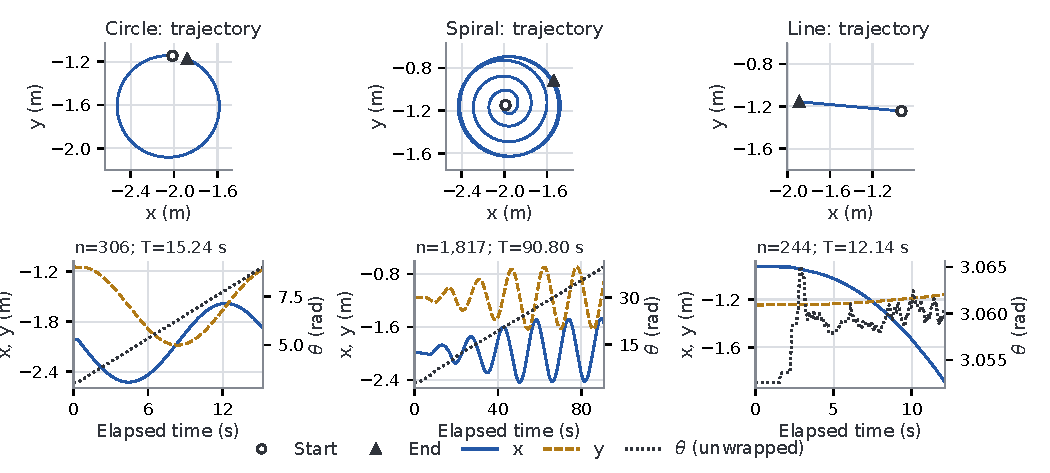
\includegraphics[width=\linewidth]{figures/odometry_results.pdf}
\caption{Odometry: equal-aspect $x$--$y$ paths (top) and position/heading histories (bottom). Left axes show metres; right axes show unwrapped radians. Each run uses its own axis ranges. Titles give sample count $n$ and duration $T$.}
\label{fig:odometry}
\end{figure}

\textbf{Circle:} The resulting radius is \odomCircleRadius~m; $\theta$ increased by \odomCircleYaw~radians during the \odomCircleDuration~s recording. Since this is less than $2\pi$~radians, a full circle was not completed.

\textbf{Spiral:} The outer-loop radius is approximately \odomSpiralRadius~m; $\theta$ increased by \odomSpiralYaw~radians during the \odomSpiralDuration~s recording. The loops initially widen, then overlap near the outer boundary as the radius becomes approximately constant.

\textbf{Line:} The path length is \odomLineLength~m over \odomLineDuration~s, with heading variation of only \odomLineYawSpan~rad (\odomLineYawDegrees$^\circ$). The increasing magnitude of the position slope indicates acceleration.

\section{IMU results and discussion}
Figure~\ref{fig:imu} shows logged IMU-frame accelerations (specific force) and $z$-axis angular rate.

\begin{figure}[H]
\centering
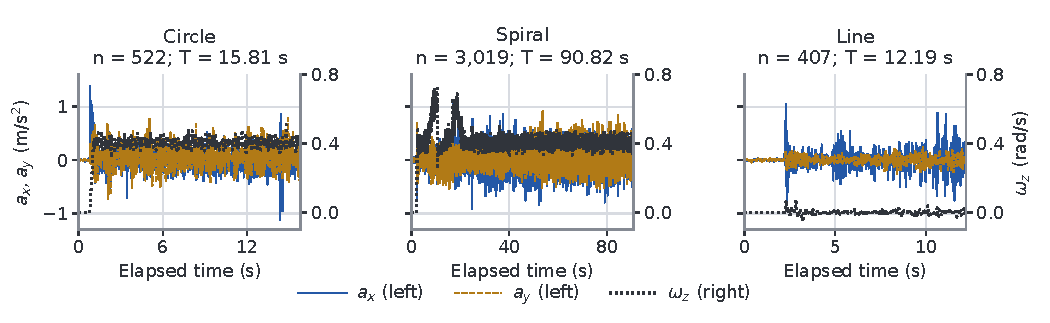
\includegraphics[width=\linewidth]{figures/imu_results.pdf}
\caption{Unsmoothed IMU samples on shared scales. Acceleration uses the left axes and angular rate the right; elapsed time starts at each file's first timestamp.}
\label{fig:imu}
\end{figure}

\clearpage
\textbf{Circle:} Mean $\omega_z$ is $0.402$~rad/s over 2--15~s of the 15.81~s recording, showing sustained turning after startup.

\textbf{Spiral:} Mean $\omega_z$ is $0.403$~rad/s over 25--90~s of the 90.82~s recording; larger early variations settle into steady turning.

\textbf{Line:} Mean $\omega_z$ is $5.4\times10^{-4}$~rad/s over 12.19~s, indicating little net rotation. The mean of $a_x$ is close to zero ($0.0017$~m/s$^2$), indicating that positive and negative readings largely balance over the recording.

\section{LiDAR results and map acquisition}
Figure~\ref{fig:lidar} uses the scan nearest each run's temporal midpoint.
Rows contain 720 ranges followed by angle metadata and timestamp.
Using original beam indices, $\alpha_i=\alpha_{\min}+i\Delta\alpha$,
$x_i=r_i\cos\alpha_i$, and $y_i=r_i\sin\alpha_i$.
Removing positive-infinity returns retains 456, 458, and 488 points.
All finite positive ranges remain because sensor limits were not logged.
Wall-like segments appear in every scan; their orientations differ in these local sensor frames.

\begin{figure}[H]
  \centering
  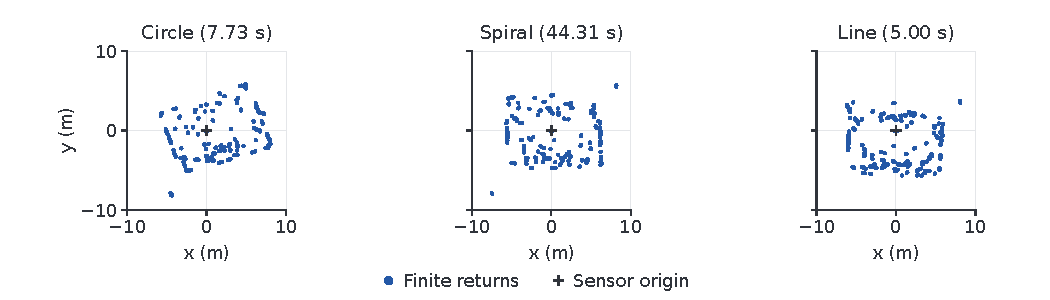
\includegraphics[width=7.0in]{figures/lidar_results.pdf}
  \caption{Midpoint LiDAR scans in their individual sensor frames; $+$ marks the sensor origin. Times are relative to each LiDAR log's first timestamp.}
  \label{fig:lidar}
\end{figure}

\noindent\begin{minipage}[t]{0.49\textwidth}
  \vspace{0pt}
  \centering
  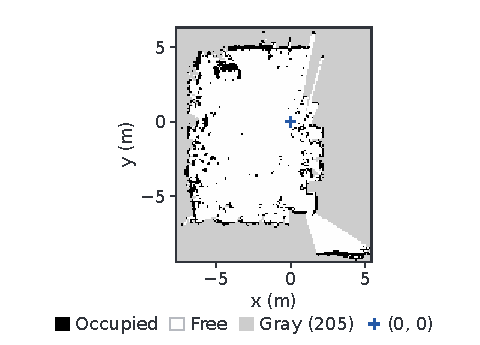
\includegraphics[width=3.2in]{figures/map_results.pdf}
  \captionof{figure}{Saved PGM map, 263$\times$315 cells at 0.05 m/cell. Lower-left origin: $(-7.72,-9.43)$ m, zero yaw.}
  \label{fig:map}
\end{minipage}\hfill
\begin{minipage}[t]{0.48\textwidth}
  \vspace{2pt}
  \raggedright
  Figure~\ref{fig:map} preserves the saved map's pixels.
  A broad free region and room boundary are visible, but scattered returns and thick, broken boundaries limit geometric precision.
  Grey unknown/intermediate cells occupy 49.3\% of the image.
  The YAML free threshold, 0.25, exceeds grey-205 occupancy $50/255\approx0.196$, so these cells would reload as free; this metadata limitation requires correction before reuse.
\end{minipage}

\medskip
\textbf{Overall Interpretation:}
\begin{list}{-}{\setlength{\leftmargin}{1em}\setlength{\labelwidth}{0.6em}\setlength{\labelsep}{0.4em}\setlength{\topsep}{2pt}\setlength{\partopsep}{0pt}\setlength{\itemsep}{1pt}\setlength{\parsep}{0pt}}
\item \textbf{Odometry:} Outputs position and heading, showing a partial circle, widening spiral loops that later overlap, and a nearly straight path with increasing speed.
\item \textbf{IMU:} Outputs sensor-frame acceleration and angular rate, indicating turning during the circle and spiral, and little net turning during the line.
\item \textbf{LiDAR:} Outputs distances at known beam angles, showing nearby surfaces. The saved map shows free space and obstacles in the environment.
\end{list}
\end{document}
